\section{Metodology and Results}

    The following subsections are about the work done in this 3rd part of the project.


\subsection*{2.1 Pump Integration}

    The pump integration in the automation algorithm bring us a new controllable variable, the Flowrate. Now we can control the spraying mode with the
    two main variables that afect the system. 
    It will bring more complexity for the system since now we are dealing with multivariable control.
    Controlling also the flowrate gives to this project a new dimension in the system giving us freedom to explore the flowrate properties.
    Our control model is now a MISO\footcite{MISO: Multiple Inputs Single Output} system. The crossover (couple) between the controlled variables will be evaluated in further reports.

    About the pump interface. As I could not find a good ready-to-use library for this pump I developed an simple and intuitive interface to be our software routine.
    The communication protocol used is RS-232. In the software routine the communication used is python serial interface. The pump commands list were found in the user manual.


\subsection*{2.2 Exploring Flowrate}

    As a first test with the new controlled variable, Flowrate a new procedure was developed. With the goal to scan the stability region of the cone jet mode through the voltage and flowrate variables.
    This procedure was implemented in the controller thread routine as a new sequence that can be configured in the setup file before an experiment.
    The algorithm of this sequence in the controller thread is shown bellow.


    \begin{algorithm}
        \caption{MAP sequence in controller thread}\label{alg:cap}
        \begin{algorithmic}
        \Procedure{MAP}{$flowrate\textunderscore values$} 
            \ForAll{flowrate\textunderscore values}  \Comment{scanning in the flowrate range}
                \State \Call{send\textunderscore flowrate\textunderscore command}{flowrate}
                \State $voltage \gets voltage\textunderscore start$
                \While{$voltage \leq voltage\textunderscore stop$} \Comment{scanning in the voltage range}
                    \State \Call{send\textunderscore voltage\textunderscore command}{voltage}
                    \State \Call{sleep}{step \textunderscore time}
                    \State $voltage \gets voltage + step\textunderscore size$
                \EndWhile
            \EndFor
        \EndProcedure

        \end{algorithmic}
    \end{algorithm}

    In the figures 5 and 6 we can see the results of this mapping experiments. The liquid used is pure ethanol. 
    Each figure has 3 graphs with shared x axis representing the samples collected. The first is the current values collected through all the experiment.
    The second is the voltage values applied in each window of data collected. The colors represent the spraying classification defined by our routine.
    The third graph shows the current mean value of each data sample.
    Note that the experiment is composed of loops that increase voltage, change flowrate and repeat.

    \begin{figure}[H]
        \center
        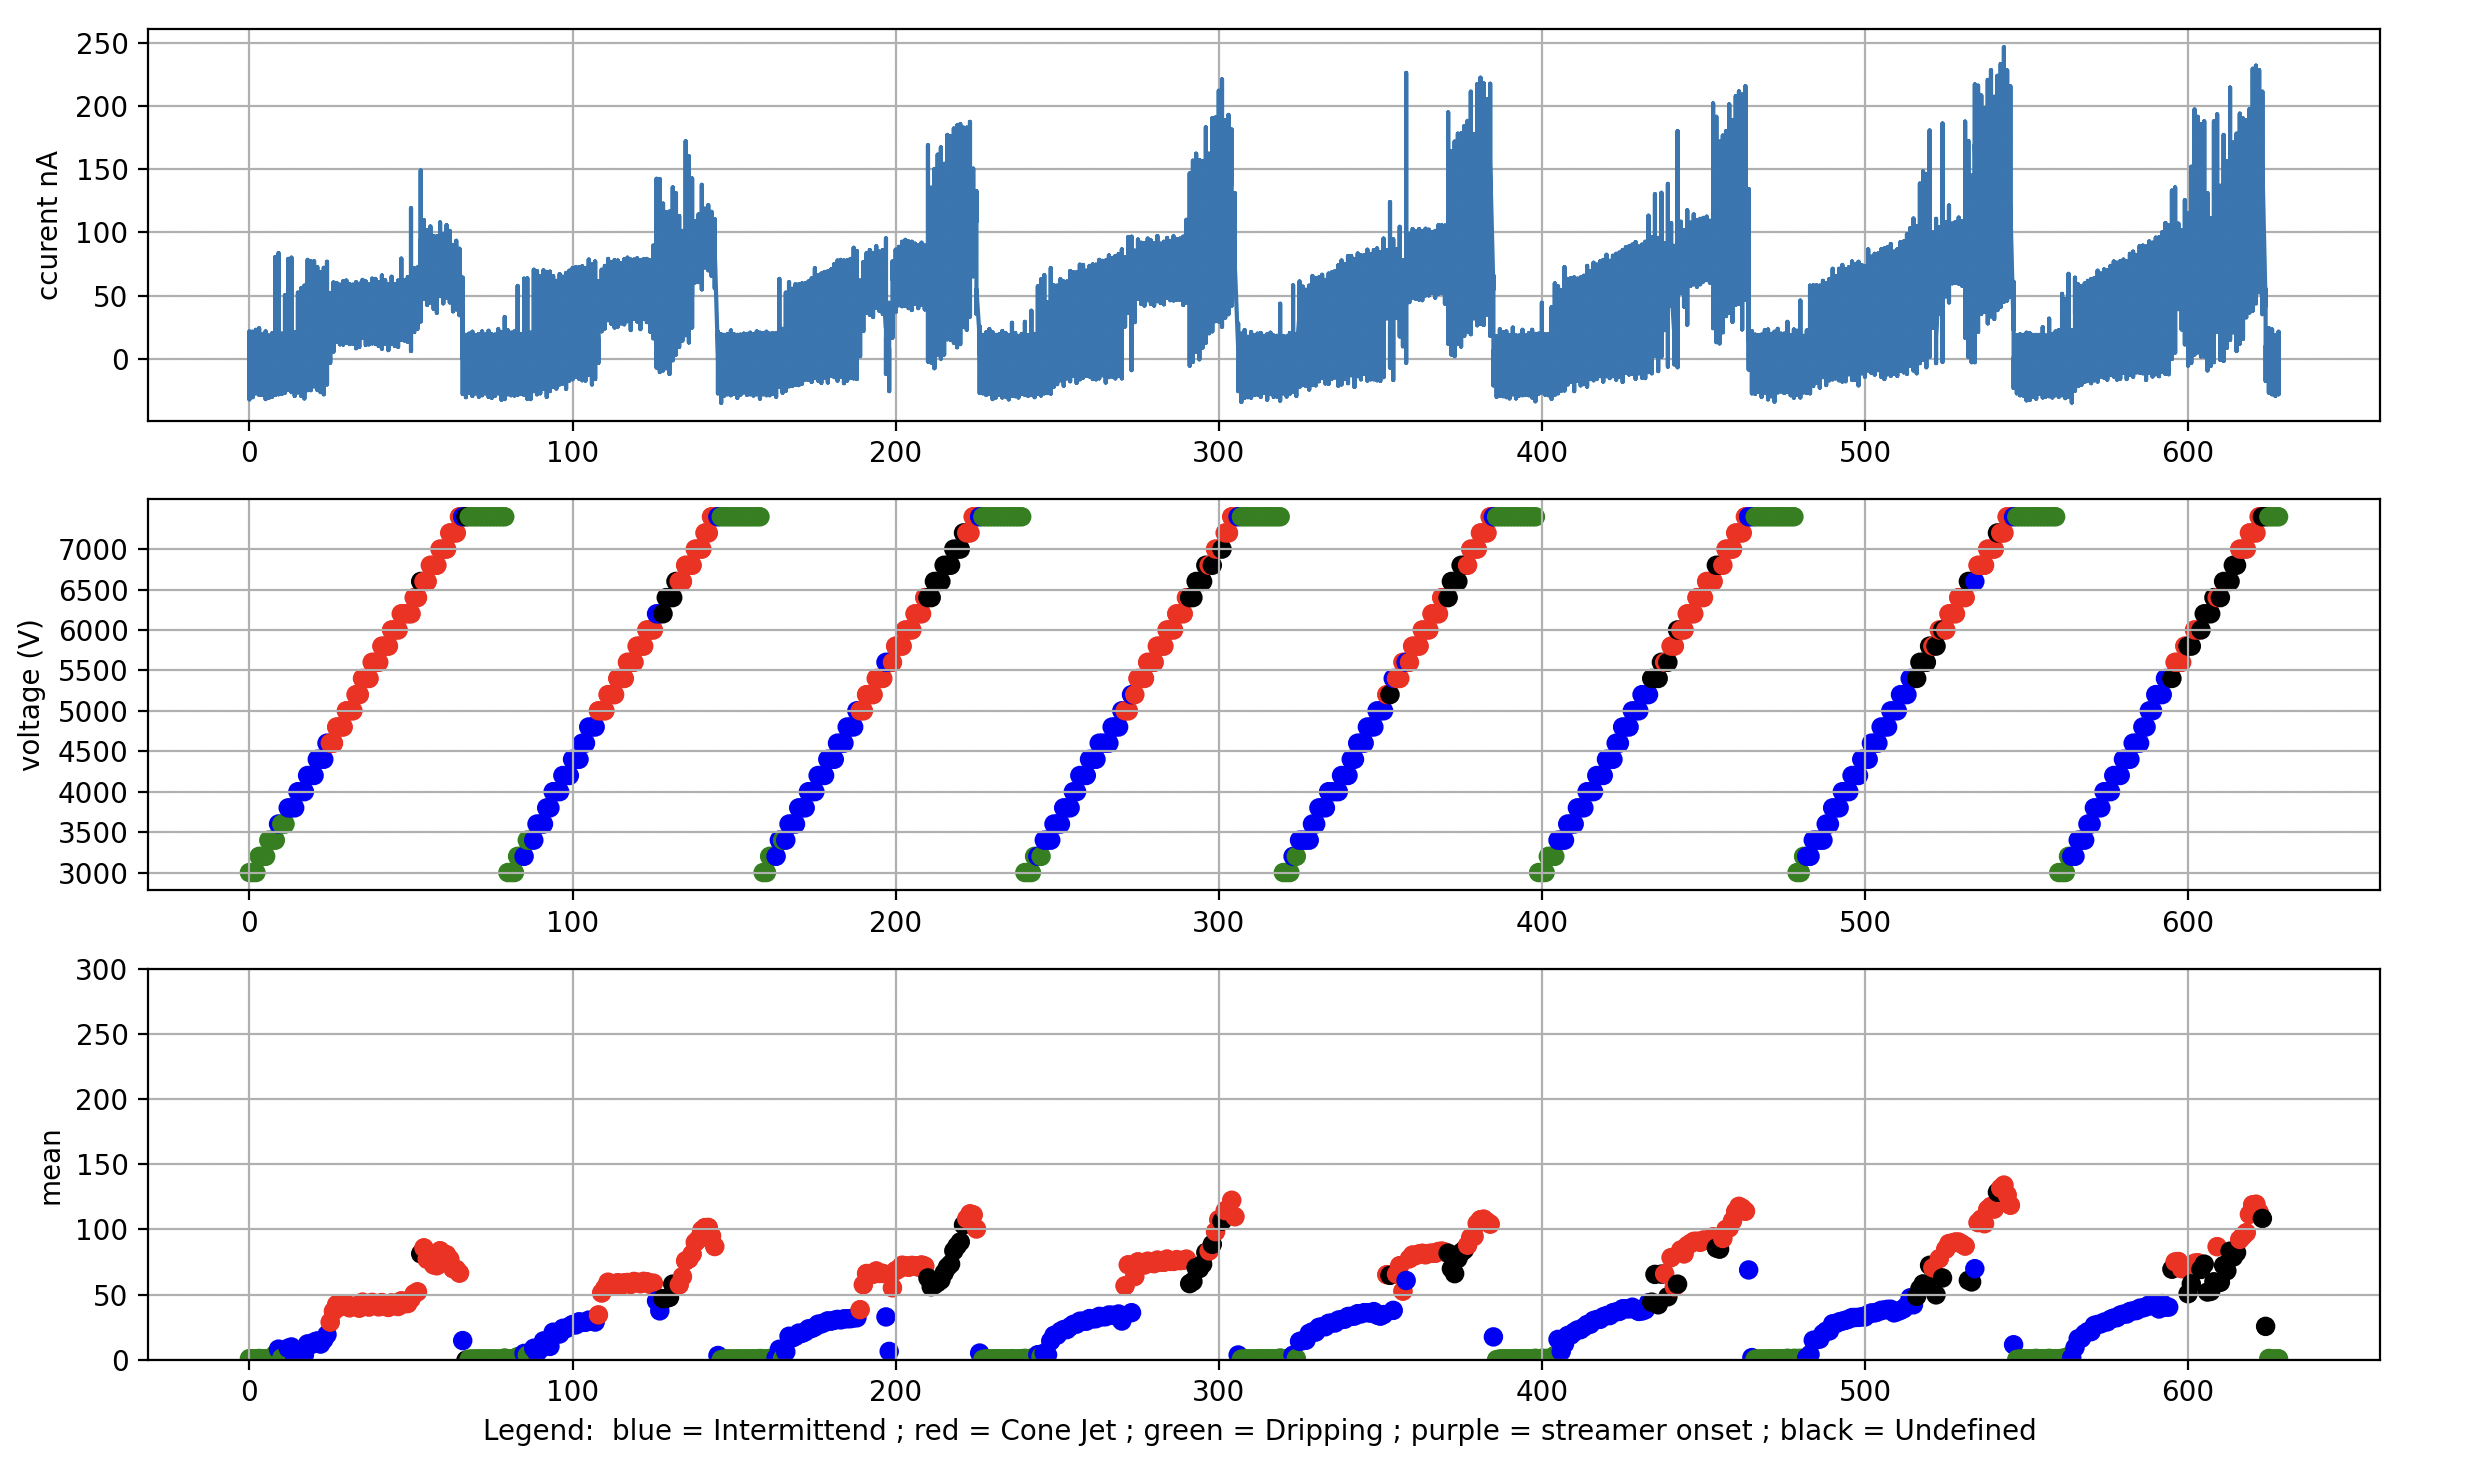
\includegraphics[width=15cm]{images/map2Data.png}
        \caption{Mapping Experiment example 1 }
    \end{figure}

    \begin{figure}[H]
        \center
        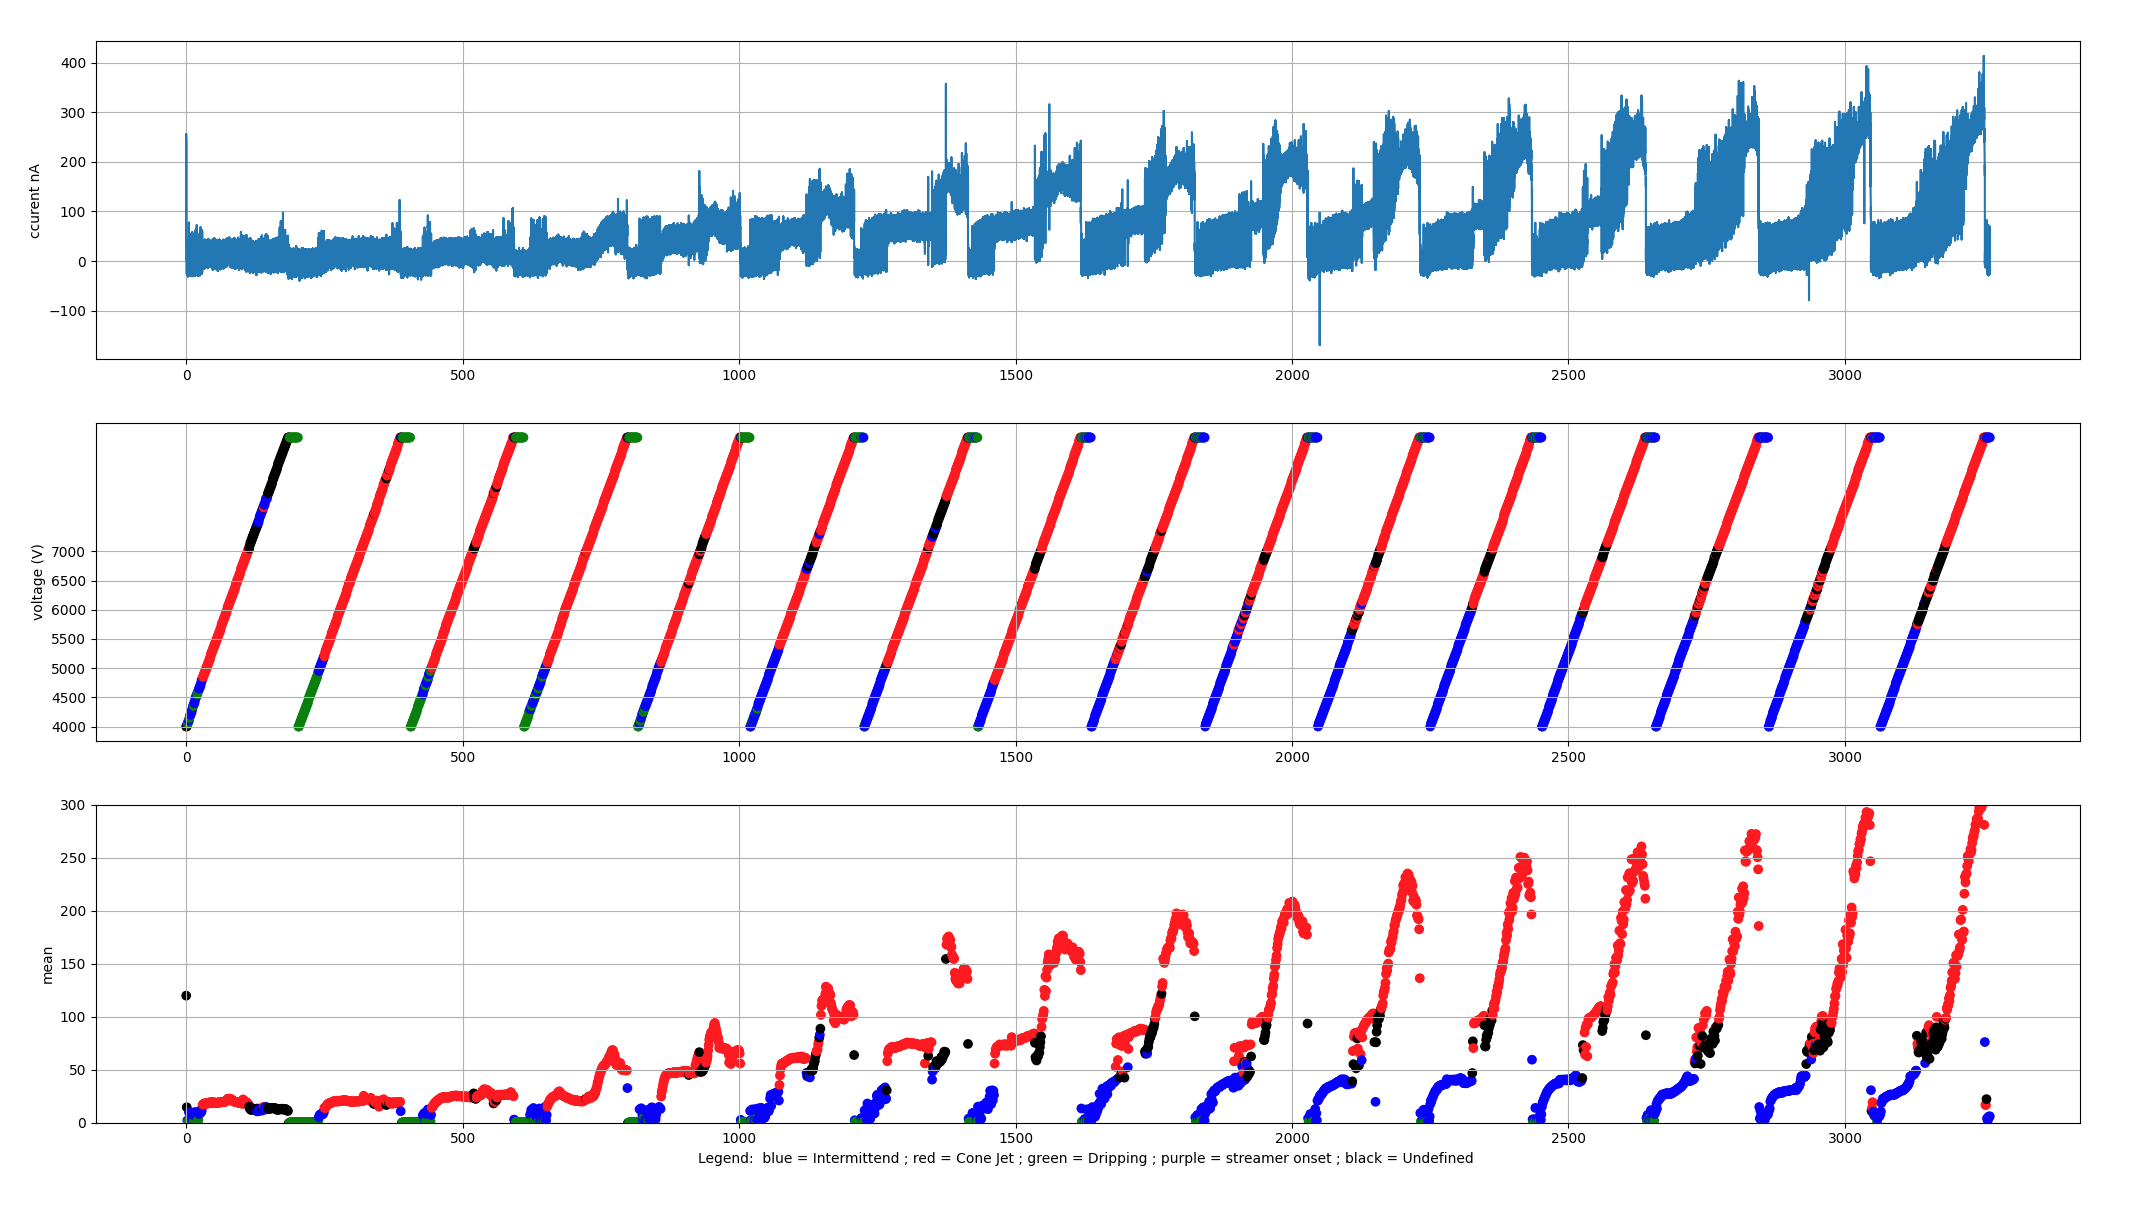
\includegraphics[width=15cm]{joao_26-01-22/graphs-exp-26-01.png}
        \caption{Mapping Experiment example 2}
    \end{figure}





\subsection*{2.3 Manual experiments}

    For better understand the effects of both voltage and flowrate in the spraying dinamycs manual experiments were made.
    Also in order to find the stability region of cone jet mode for the liquid and setup used.


        \begin{figure}[H]
            \center
            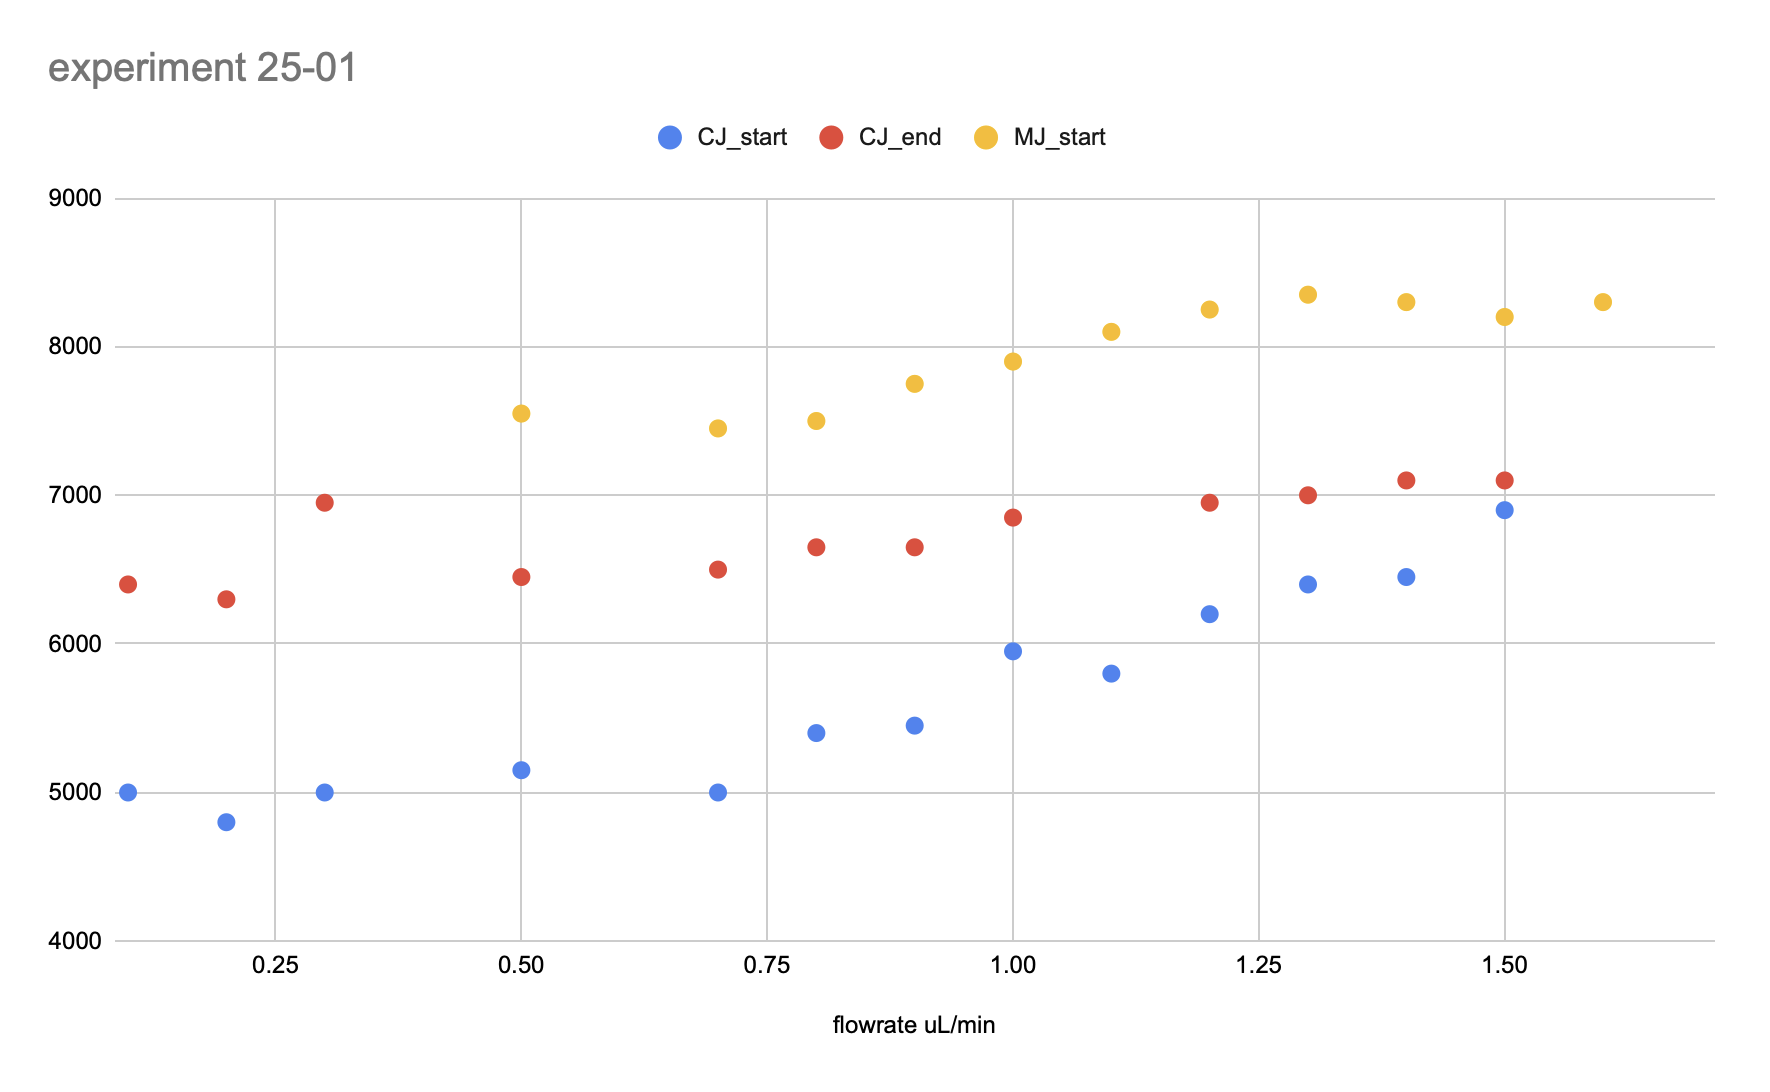
\includegraphics[width=12cm]{joao_26-01-22/exp25-01-1.png}
            \caption{ exp25-01-1 (V x Q)}
        \end{figure}

        \begin{figure}[H]
            \center
            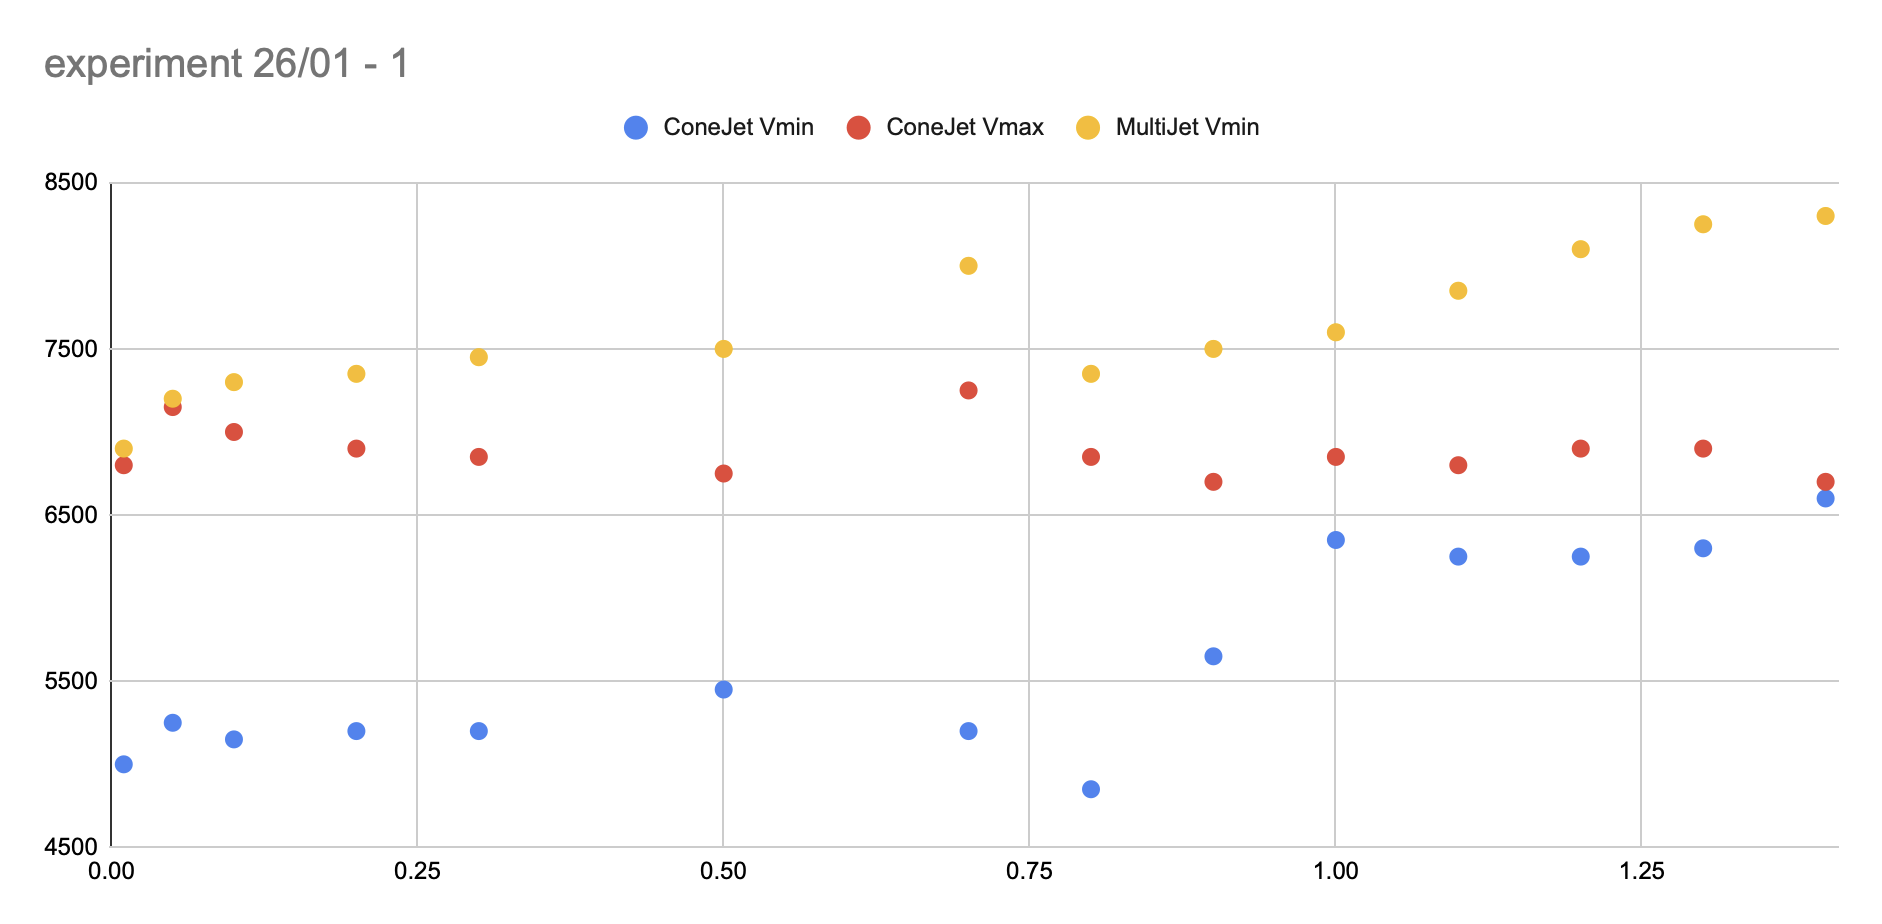
\includegraphics[width=12cm]{joao_26-01-22/exp-26-01-1.png}
            \caption{ exp-26-01-1 (V x Q)}
        \end{figure}

        \begin{figure}[H]
            \center
            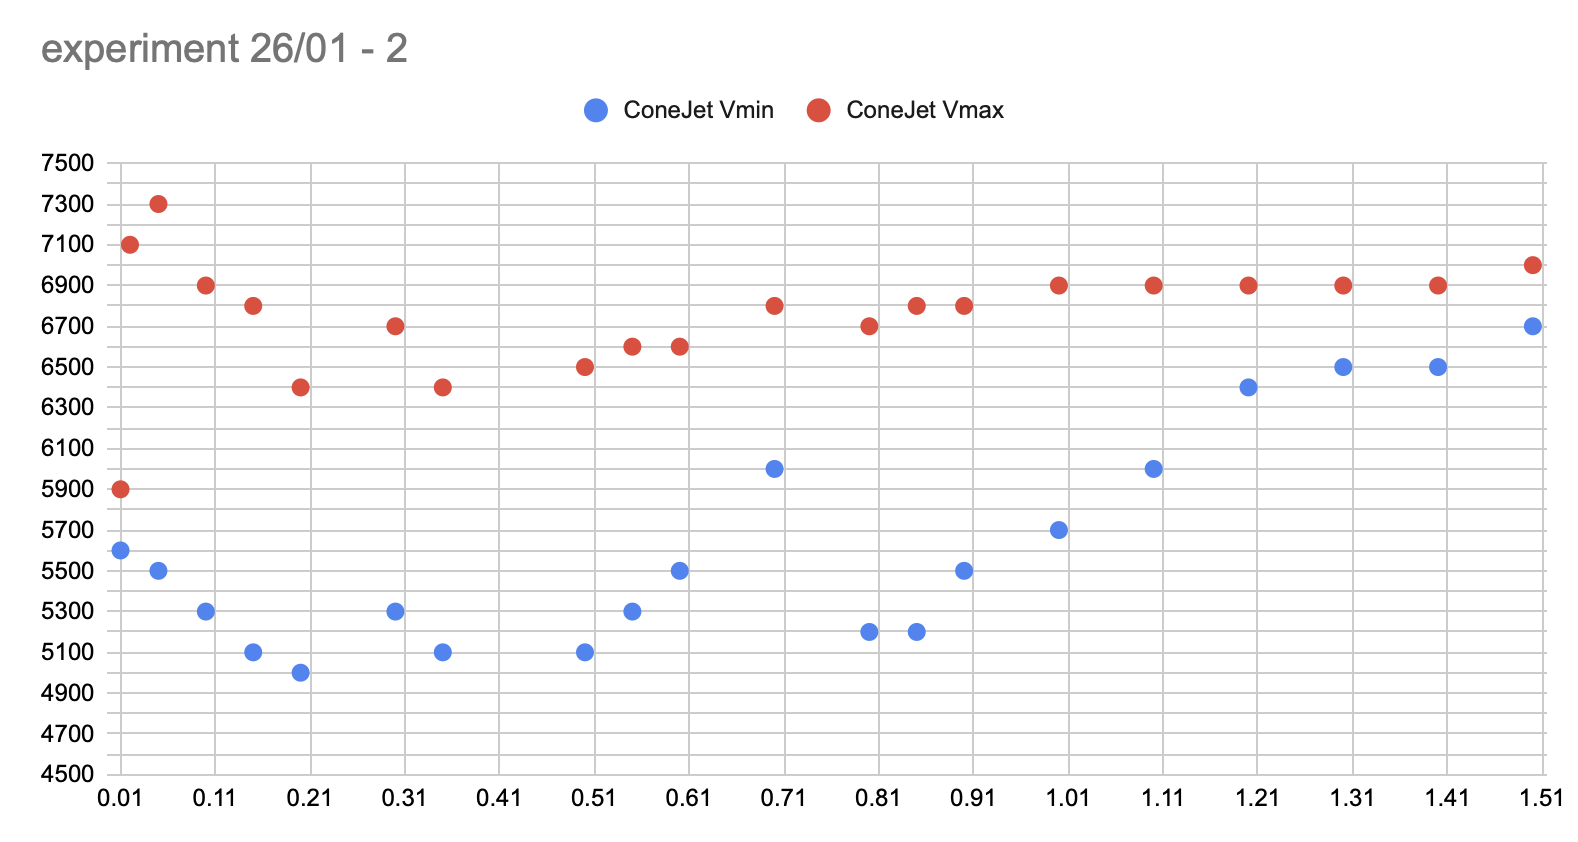
\includegraphics[width=12cm]{joao_26-01-22/exp26-01-2.png}
            \caption{ exp-26-01-2 (V x Q)}
        \end{figure}


\subsection*{2.4 Automatic experiments}

    With the desired voltage and flowrate range defined for the automatic experiment the next part is to define how many datapoints will be collected in both
    x and y axis. Since we are introducing a new dimension for our experiment it is also increasing fast the amount of data collected.
    The goal of this part is to find the ideal combination of voltage step size, voltage step time and flowrate step size in order to get the most accurate results without exceding the separate memory for each experiment.
    
    In the further improvements of the routine it's ideal to apply a real time file writing with all experiment data.
    This will prevent that any crashes in the program lose all data and not overflow the memory allocated for the program.


    \begin{multicols}{3}


        \begin{figure}[H]
            \center
            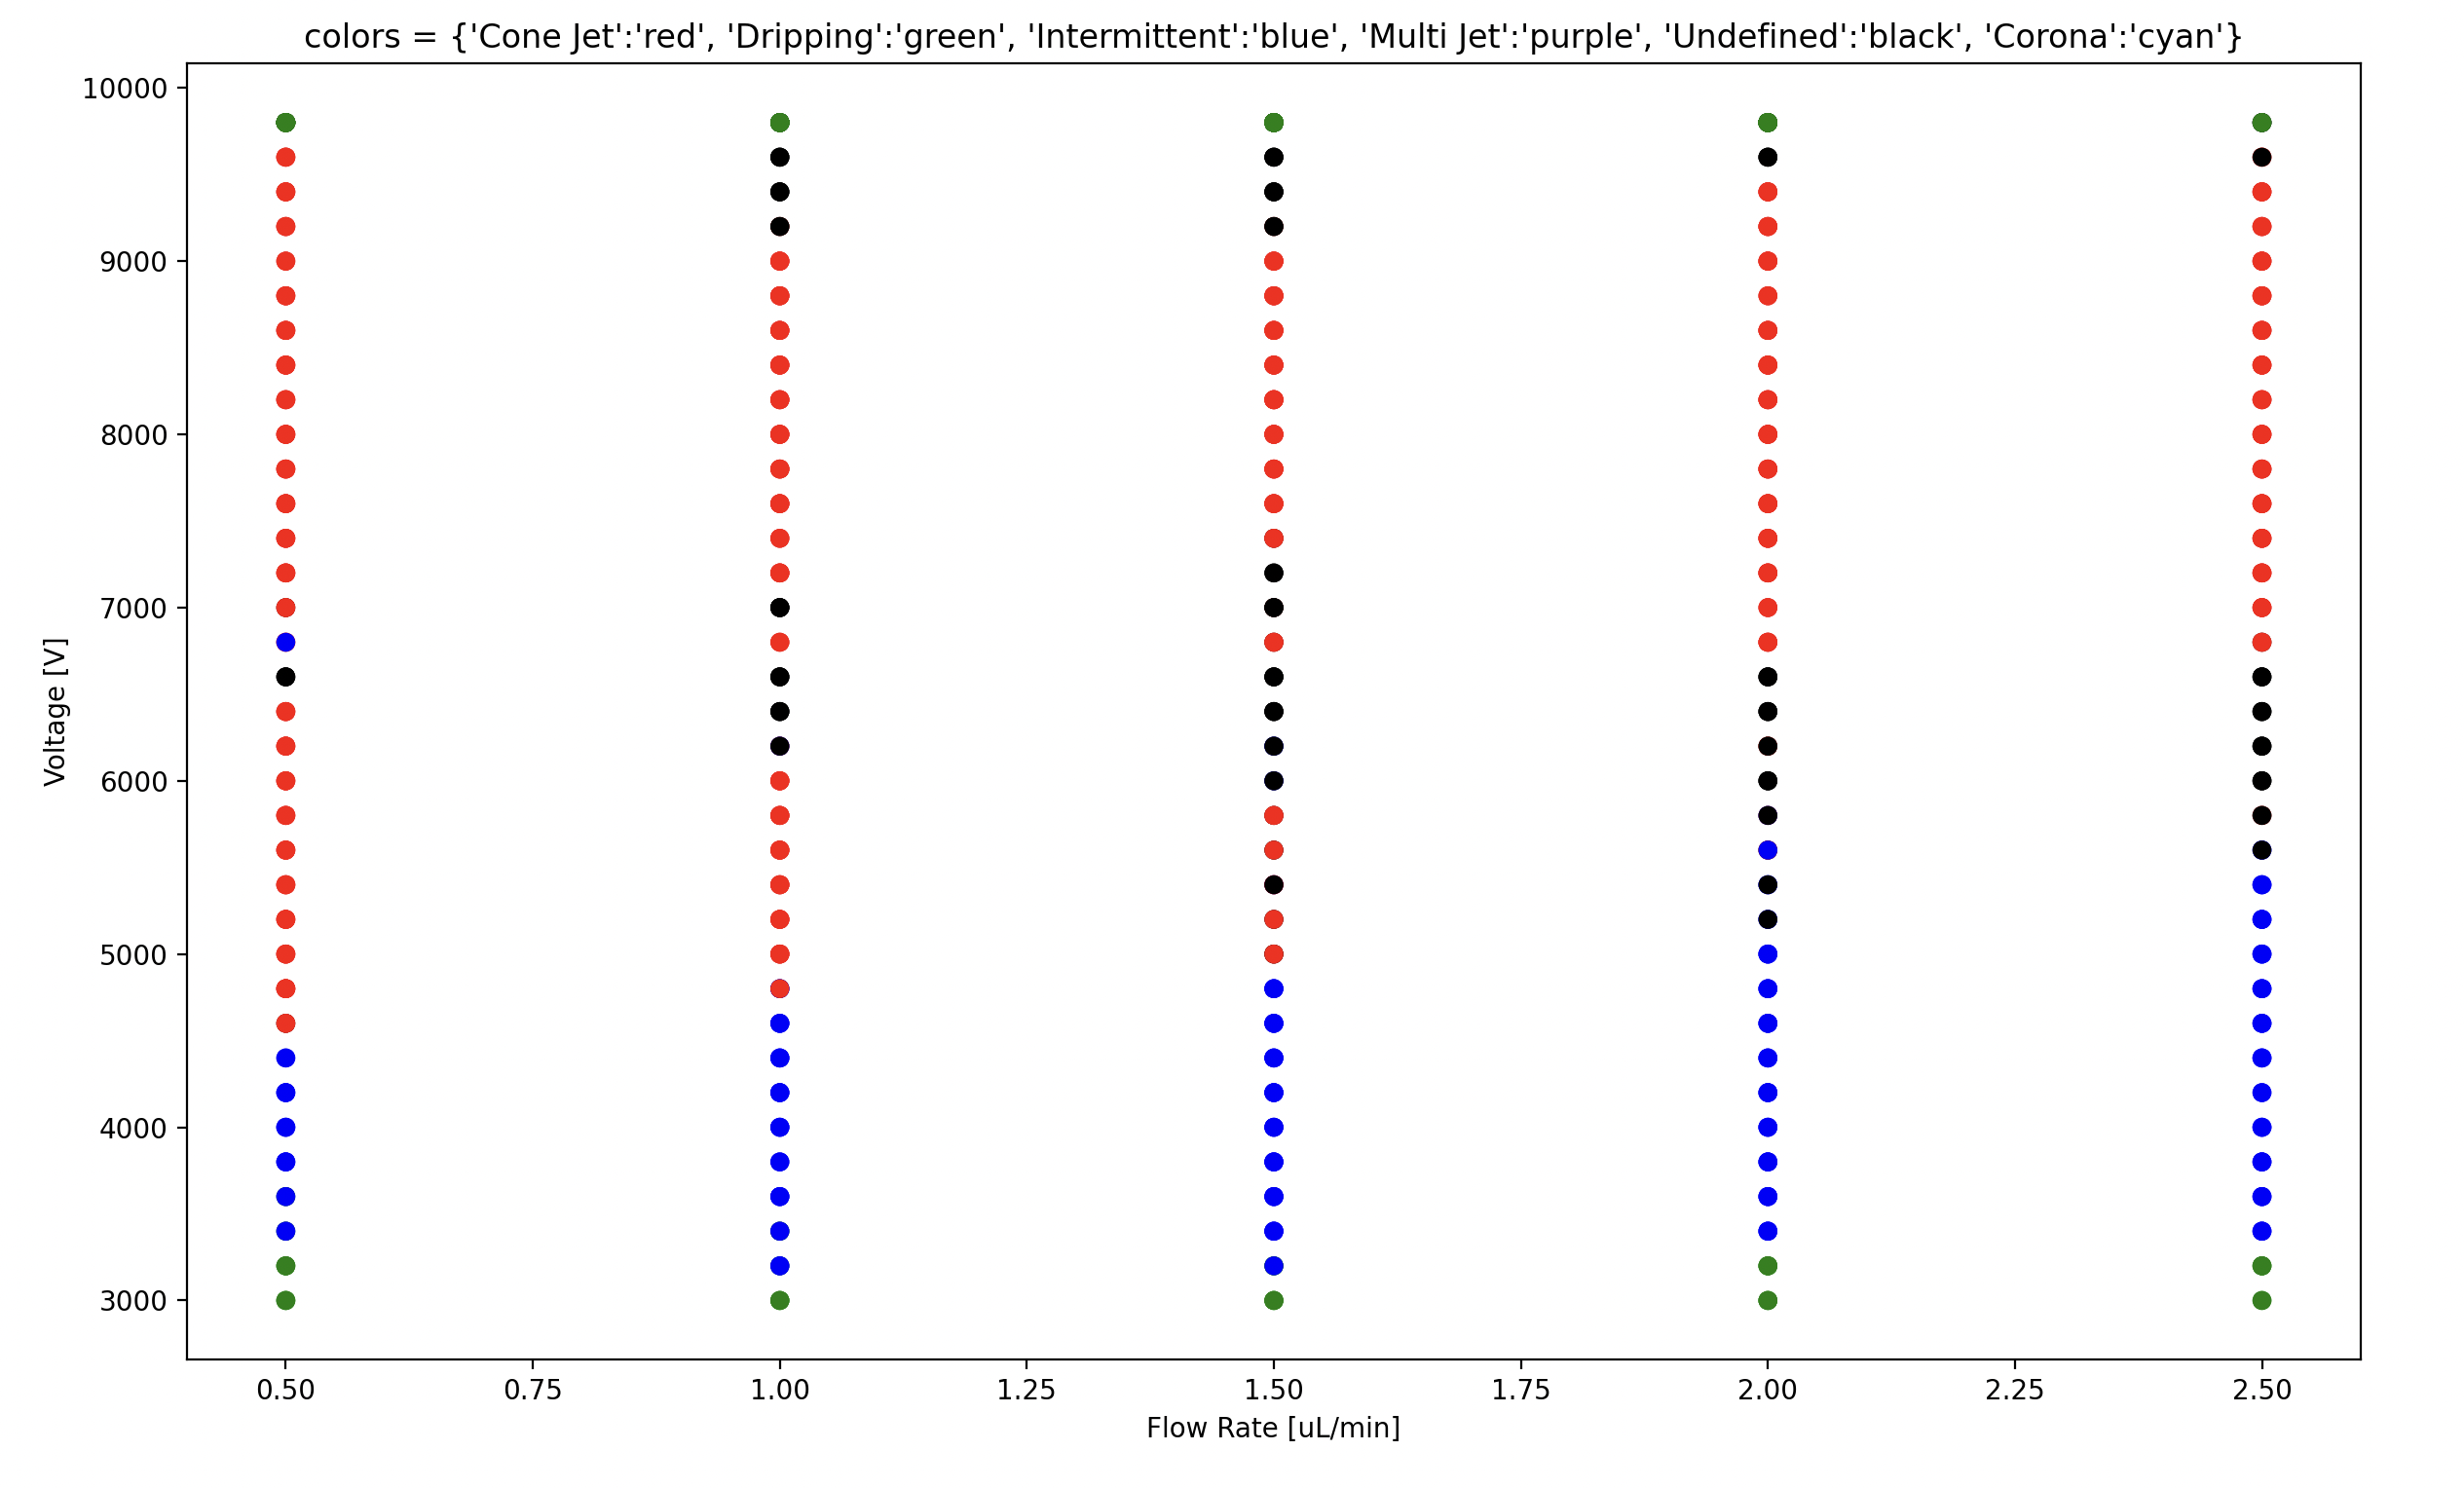
\includegraphics[width=5cm]{images/map1.png}
            \caption{First mapping trial}
        \end{figure}

        \begin{figure}[H]
            \center
            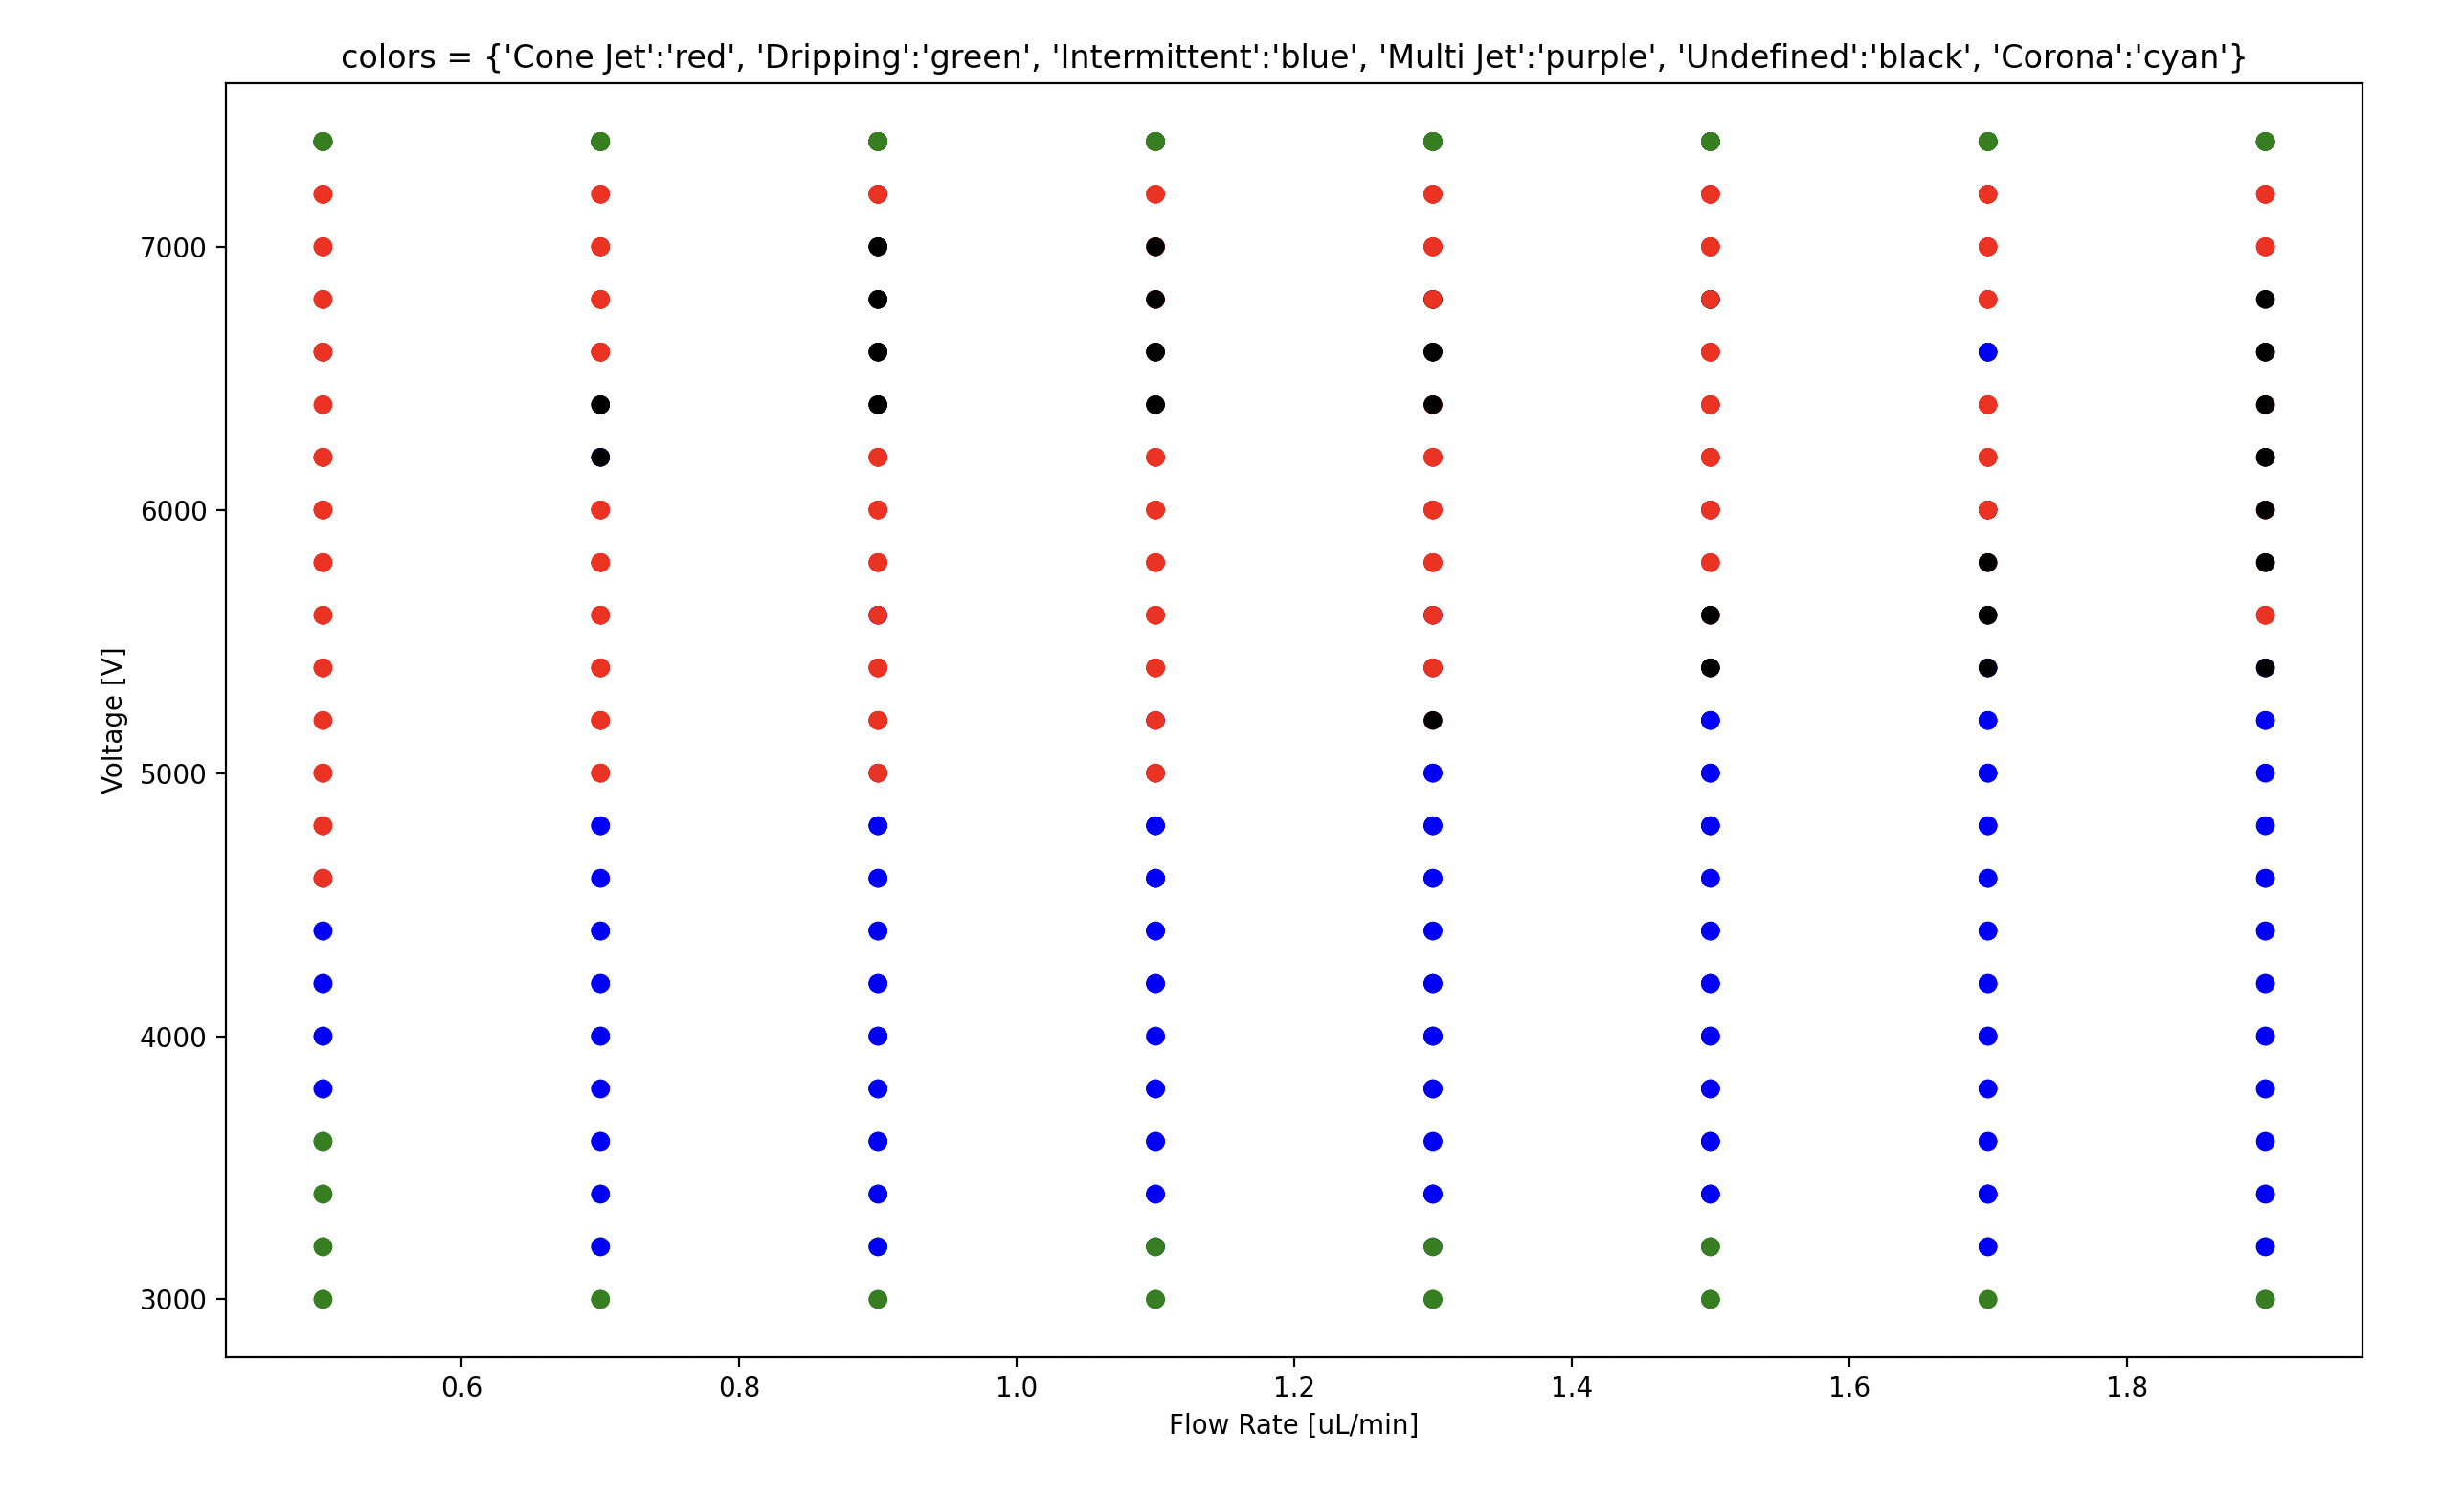
\includegraphics[width=5cm]{images/map2.png}
            \caption{Second mapping trial}
        \end{figure}


        \begin{figure}[H]
            \center
            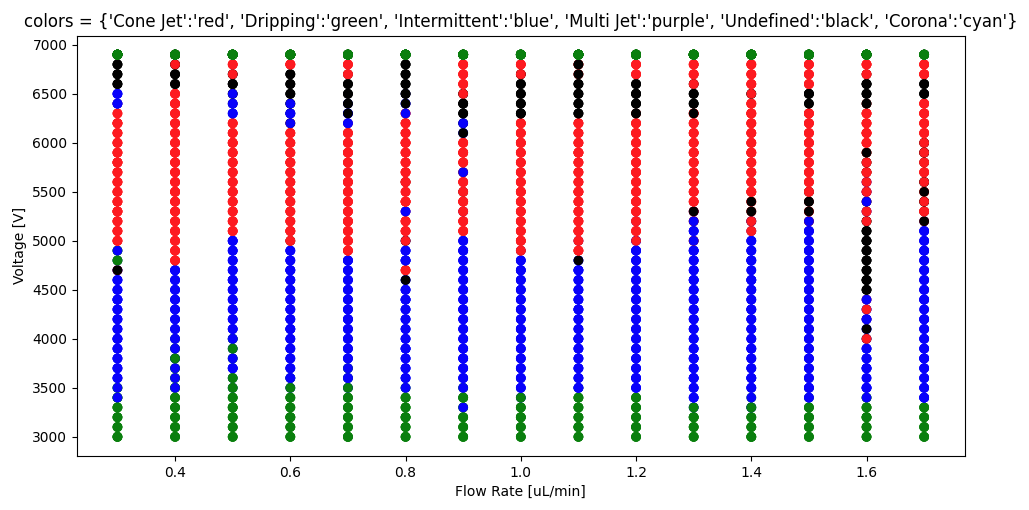
\includegraphics[width=6cm]{images/map3.png}
            \caption{third map - better result}
        \end{figure}

    \end{multicols}



\subsection*{2.5 Manual x Automatic Cone Jet stability island maps}

    For validation of the automatic system and classification some experiments were made having both manual and automatic data collecting.

    The Figure 13 shows a printscreen of how the experiment looks like in real time.
    We can see the image generated by the camera in the back.
    The routine code running in pycharm software on the right.
    And also real time signal plottings of the current data on the left.

    \begin{figure}[H]
        \center
        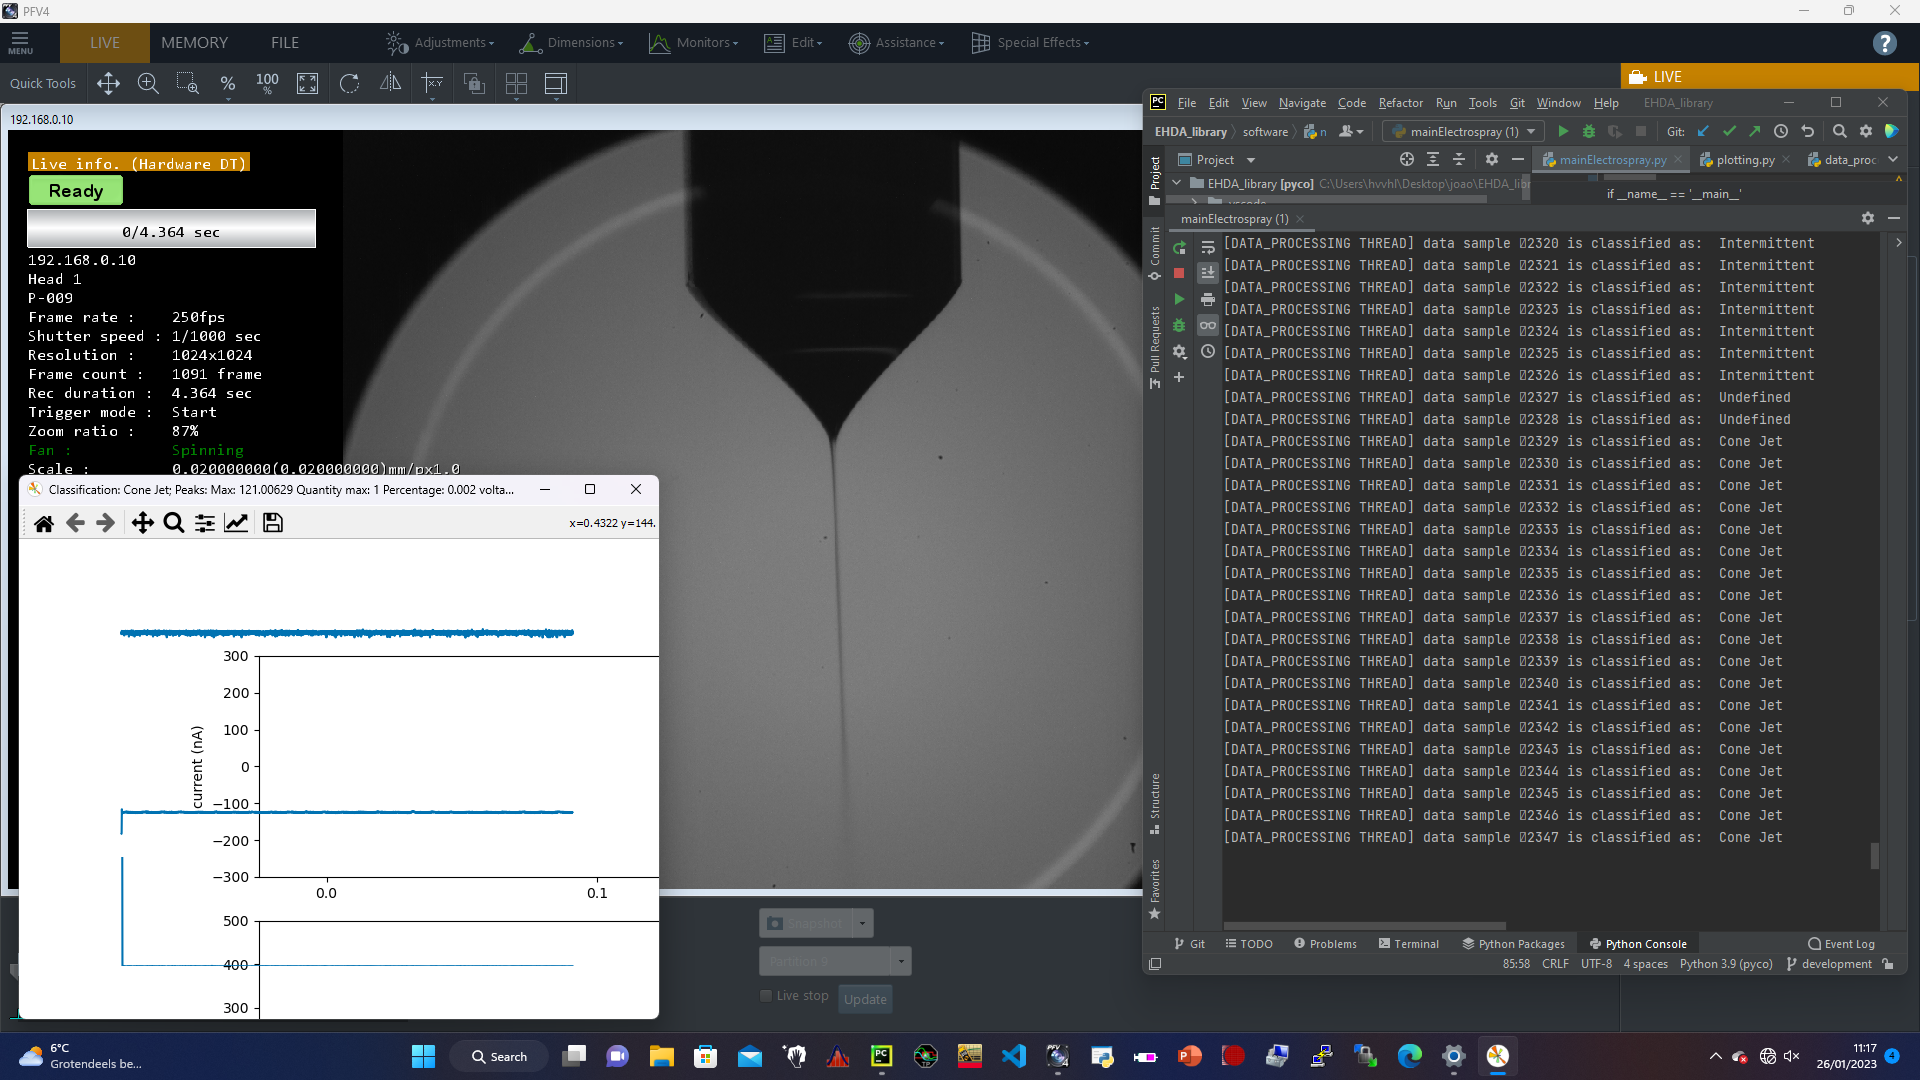
\includegraphics[width=17cm]{joao_26-01-22/screenshots/stableConeExp.png}
        \caption{running experiment print screen}
    \end{figure}

    In Figure 14 we can see a result of the map generated by the automatic classification in this experiment.

    \begin{figure}[H]
        \center
        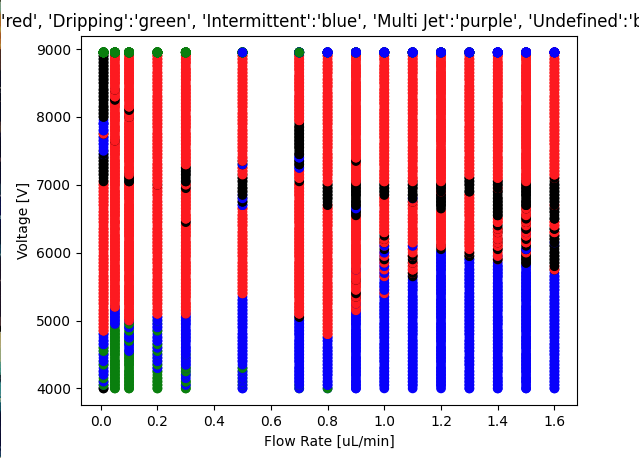
\includegraphics[width=10cm]{joao_26-01-22/map-exp-26-01.png}
        \caption{ exp-26-01-23 }
    \end{figure}

    \pagebreak

    Figures 15 and 16 shows that we could achieve a stable cone jet region map with similar shape and values in both manual and automatic classification of the same experiment.

    \begin{multicols}{2}


        \begin{figure}[H]
            \center
            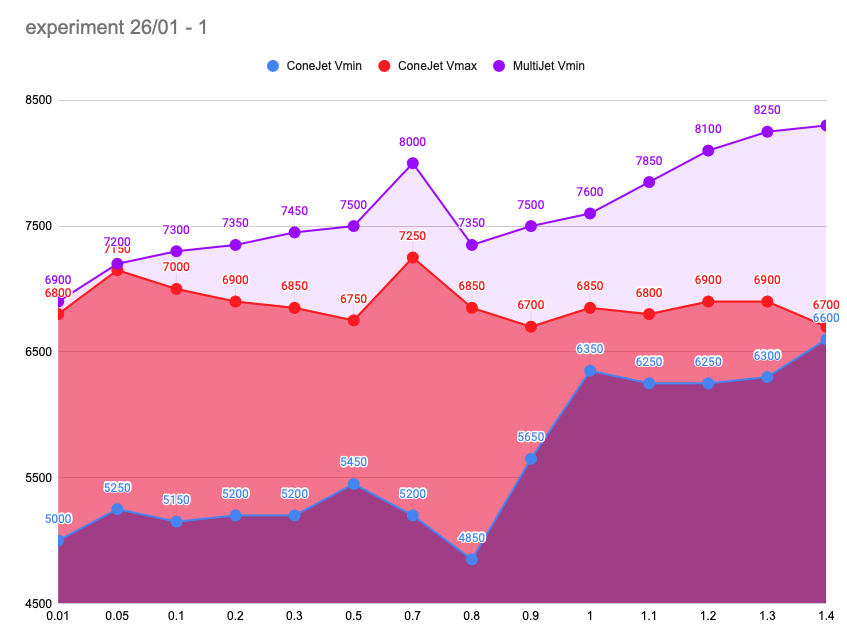
\includegraphics[width=9cm]{joao_26-01-22/manual-mapping.png}
            \caption{ exp-26-01 manual classification}
        \end{figure}

        \begin{figure}[H]
            \center
            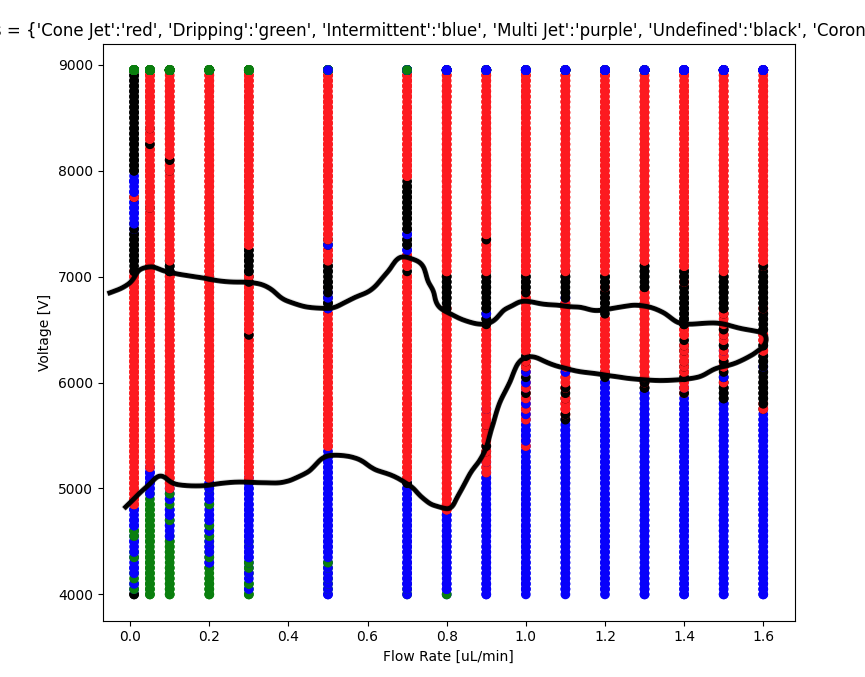
\includegraphics[width=9cm]{joao_26-01-22/map4-stabilityIsland.png}
            \caption{ exp-26-01 automatic classification}
        \end{figure}

    \end{multicols}


\subsection*{2.6 Pump machine and stepper motor noise}

    It was noticed that the motor of the pump in certains speed generate a noise caused by the stepping from the stepper motor.
    This noise from the motor was being acquired by the current data and was interfering in the classification method.
    Because of that the firsts results of the map have a lot of undefined or incorrect classifications.
    This can be reduced inserting a air bubble in the syringe to atenuate mechanical noises applied.
    Also was found a command that can be send to the pump machine to activate microstepping in the stepper motor.
    Both of this changes were made in order to add the pump machine to the system.



\subsection*{2.7 Capacitance of the system in step response}


    We had discussions if the voltage step implies in a transient state in the current acquired.
    If yes, the data acquired in this transient should not be used in the classification step. Since we want to analise
    the spraying in a constant dynamics.

    For that I reproccessed all raw data acquired cutting the head of the data window. The new classification map is showed in the figure 10.
    Also tested cutting the tail of the data window to see if have improvements in the classification.

    \begin{multicols}{2}
        \begin{figure}[H]
            \center
            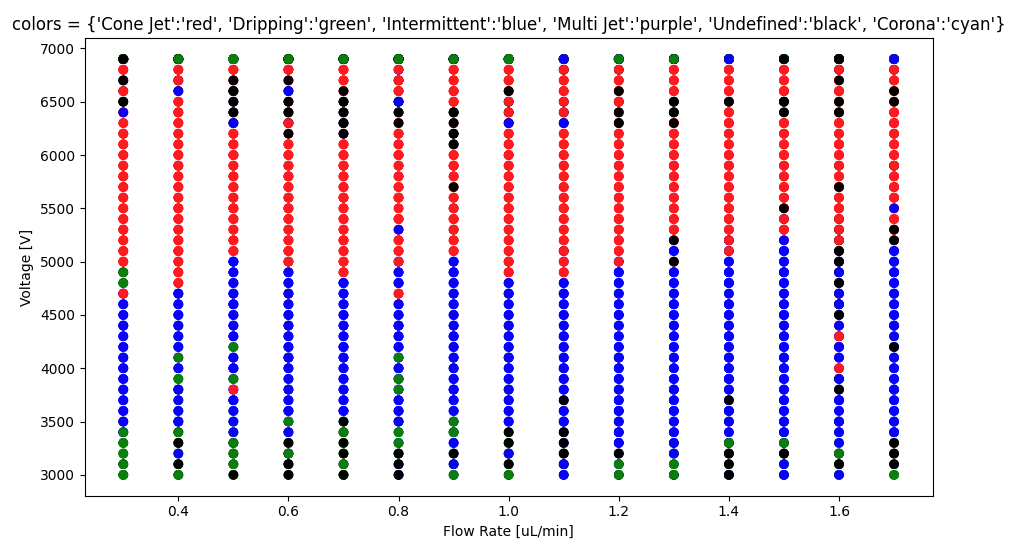
\includegraphics[width=7cm]{images/map3_reproccessed_data_head.png}
            \caption{ map3 reproccessed data head }
        \end{figure}


        \begin{figure}[H]
            \center
            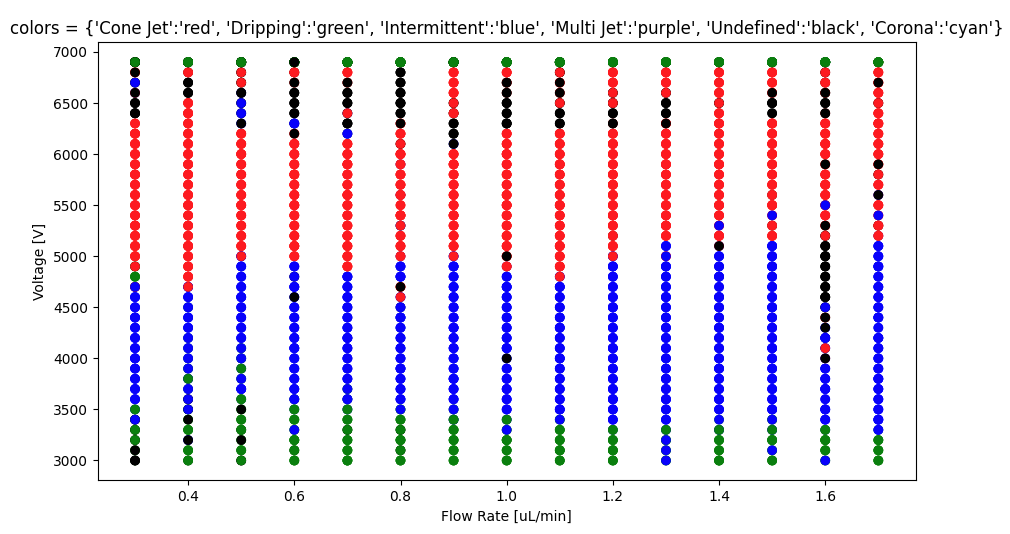
\includegraphics[width=7cm]{images/map3_reproccessed_data_tail.png}
            \caption{ map reproccessed data tail }
        \end{figure}

    \end{multicols}

    After noticing that cutting out the data collected in the transient of the step voltage did not bring any improvements to the classification.
    In the Figure 20 we see 3 random samples of current data in the experiment and there's no transient shown in the current data.

    \begin{figure}[H]
        \center
        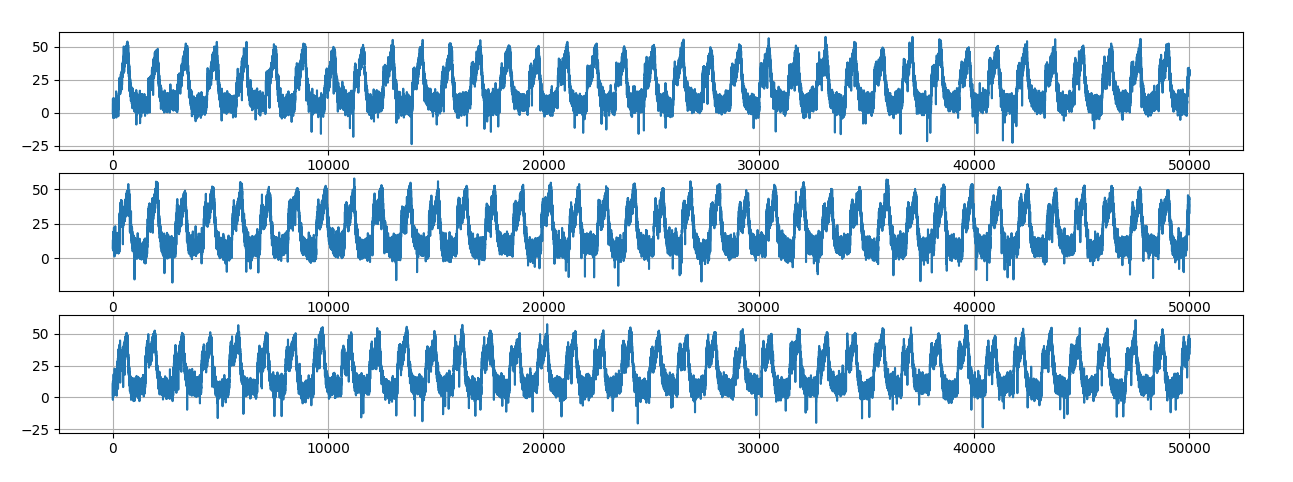
\includegraphics[width=8cm]{images/random_samples.png}
        \caption{ 3 samples of current data }
    \end{figure}

    As a conclusion of this discussion we got that with voltage steps under 250V the system does not show a transition dynamic. 
    For steps above this value we can see a capacitance curve in the current data. This is explained by the system capacitance which resists to fast changes in eletric potential.
    This treshold value of 250V will vary depending on the resultant capacitance of setup used.


\subsection*{2.8 Temperature and Humidity influences}

    During this time it was noticed that breaks in beetween the experiments was getting different results for the same setup. This can be caused by the temperature and humidity effects on the system.
    For that I included the sensor DHT11 in the system setup and software routine to collect data of this two variables. Also closed the system chamber and sprayed pure oxygen O2 to decrease the humidity inside.
    

